\documentclass[10pt]{article}
\usepackage[margin=0.7in]{geometry}
\usepackage[T1]{fontenc}
\usepackage{graphicx}
\begin{document}
\section*{Signed word composition: source derivation}
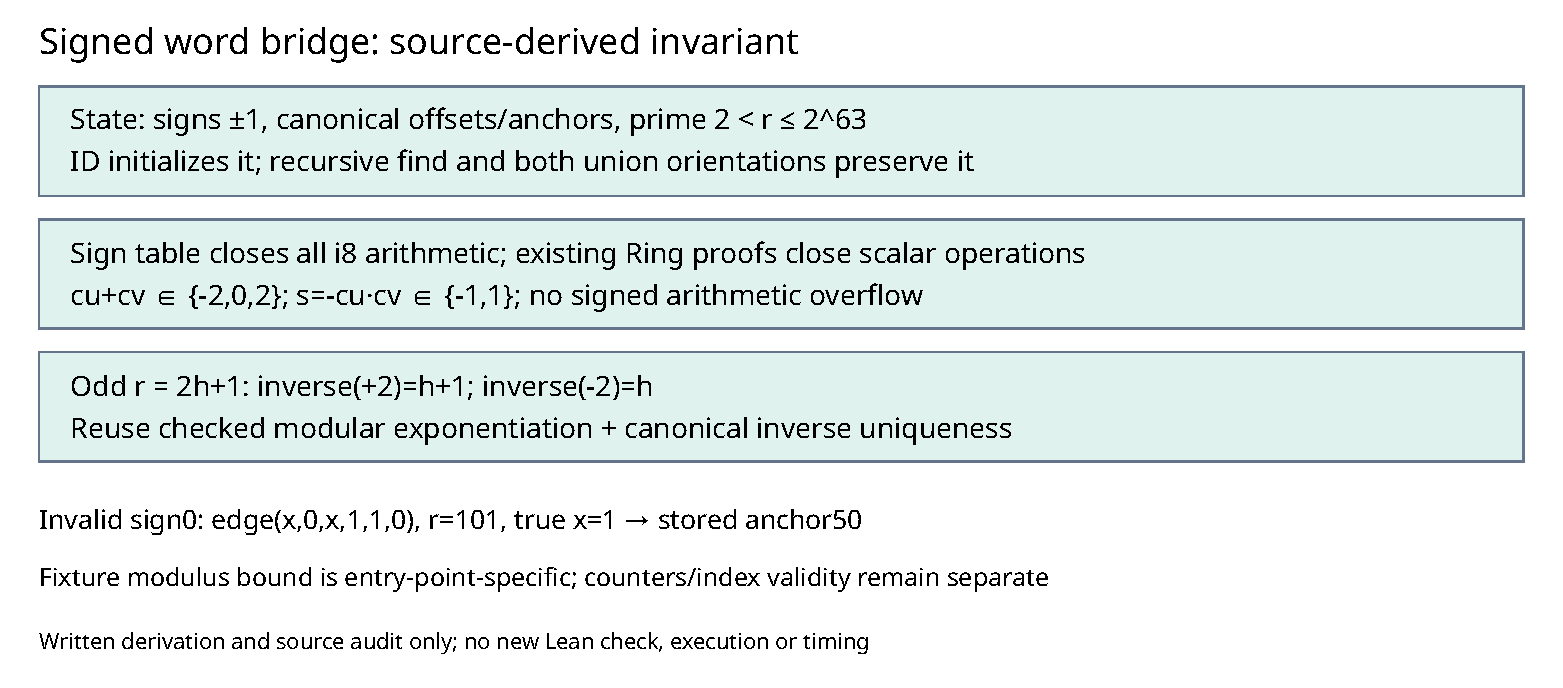
\includegraphics[width=\linewidth]{flow.pdf}

The machine bridge reduces to a finite sign invariant plus existing scalar arithmetic. For odd $r=2h+1$, the canonical inverses of $+2$ and $-2$ are $h+1$ and $h$. This is a written source-bound derivation, not a new Lean acceptance claim.

\paragraph{Preservation.}
ID initializes sign1 and zero offsets. Find multiplies signs and composes canonical offsets through signed/add. Union uses $s=-c_uc_v$ and reverses offsets using $-s$; all these signs remain $\pm1$. The sum $c_u+c_v$ is exactly $-2,0,2$, so i8 arithmetic cannot overflow. Existing GraphRingWord lemmas handle canonical add/sub/neg/widened multiplication at $r\leq2^{63}$. Anchor transport preserves canonical pairs.

\paragraph{Inverse simplification.}
Since $2(h+1)=r+1$ and $(-2)h=1-r$, the canonical inverse representatives are $r/2+1$ and $r/2$. Both fit a word without forming $r+1$. Existing generated-inverse correctness and uniqueness identify native modpow output with these values. This makes no change to runtime or counters.

\paragraph{Counterexample to omitted sign premise.}
Let $r=101$, true root value $x=1$, and call edge$(x,0,x,1,1,0)$. The incoming equation is true, but the source takes the nonzero same-root branch, chooses denominator99, inverse50, and stores anchor$(50,0)$. Collector sites construct only $\pm1$; the public edge interface does not enforce that premise.

\newpage
\section*{Caller scope and concrete obligations}
\paragraph{Actual source.}
three\_leads.rs1543--1579 initializes signs;1582--1597 composes find;1658--1711 reduces edges and updates union/anchors. Its collector constructs signs at1908--1921. The frozen Kummer Adapter graph.rs11 also constructs only $\pm1$. The fixture original\_gstep\_fixture in pruned.rs814 asserts $2\leq r\leq2^{63}$, then asserts canonical labels before doubling. That guard belongs to this fixture, not every entry point in the file.

\paragraph{Bounds.}
For canonical inputs, $a+b\leq2r-2<2^{64}$ at $r\leq2^{63}$. Above that bound the maximal canonical pair overflows. Noncanonical inputs defeat literal Ring.neg because it subtracts before reducing; signed$(+1,a)$ returns $a$ unchanged. The field theorem therefore needs exact sign and canonical-word premises. Counter/size headroom and valid array indices remain separate.

\paragraph{Next checked interface.}
Extend mutable graph state with GoodWords and prove native word-Run preservation/refinement using existing scalar lemmas and the four-entry sign table. Extend edge to preserve that predicate in both union orientations and the same-root branch. Then compose decoded state with same\_after\_two\_finds and canonical equality reflection. Specialize existing inversion to the closed half-modulus values. The collector still supplies its geometric true-edge certificate.

\paragraph{Evidence and status.}
REPORT.md contains the full written induction and precise source mapping. obligations.json records eight interfaces and their present status; source-bindings.sha256 pins inspected files. The GraphRing packet has historical Python-gate provenance and is read as an existing proof dependency; this audit does not re-certify that workflow. No code compilation, formal replay, timing, scientific execution, repository edit or cloud operation occurred.
\end{document}
